%
\documentclass[10pt,a4paper]{article}


\usepackage{array}
\usepackage{subfigure}
\usepackage{graphicx}
\usepackage{amssymb}
\usepackage{amsmath}
\usepackage{cite}
\usepackage{color}
\usepackage{url}
\usepackage[lined,linesnumbered,ruled,norelsize]{algorithm2e}
\usepackage{listings}
\lstset{
  language=Octave, 
  basicstyle=\footnotesize, 
  frame=single, 
  showspaces=false, 
  showstringspaces=false}




\begin{document}

\title{Experiment 6: SVM Linear Classification}

\maketitle
  
\section{Description}
%
  This exercise gives you practice with using SVMs for linear classification. You will use a free SVM software package called LIBSVM that interfaces to MATLAB/Octave. To begin, download the LIBSVM Matlab Interface (choose the package with the description ``a simple MATLAB interface'') and unzip the contents to any convenient location on your computer.

  Then, download the data for this exercise: ex6Data.zip.


\section{Installing LIBSVM}
%
  After you've downloaded the LIBSVM Matlab Interface, follow the instructions in the package's README file to build LIBSVM from its source code. Instructions are provided for both Matlab and Octave on Unix and Windows systems.

  If you've built LIBSVM successfully, you should see 4 files with the suffix ``mexglx'' (``mexw32'' on Windows). These are the binaries that you will run from MATLAB/Octave, and you need to make them visible to your working directory for this exercise. This can be done in any of the following 3 ways:
  %
  \begin{enumerate}
    \item Creating links to the binaries from your working directory
    %
    \item Adding the location of the binaries to the Matlab/Octave path
    %
    \item Copying the binaries to your working directory.
  \end{enumerate}




\section{Linear classification}
%
  Recall from the video lectures that SVM classification solves the following optimization problem:
  %
  \begin{displaymath}
    \min_{w,b}\qquad\left\Vert w\right\Vert ^{2}+C\sum_{i}^{m}\xi_{i}
  \end{displaymath}
  %
  \begin{eqnarray*}
    \mbox{subject to}\qquad y^{(i)}(w^{T}x^{(i)}+b) & \geq & 1-\xi_{i},\qquad i=1,2...,m\\
    \xi_{i} & \geq & 0,\qquad i=1,2...,m
  \end{eqnarray*}
  %
  After solving, the SVM classifier predicts ``1'' if  $w^T x + b \geq 0$ and ``-1'' otherwise. The decision boundary is given by the line $w^T x + b = 0$.




\section{2-Dimensional classification problem}
%
  Let's first consider a classification problem with two features. Load the ``twofeature.txt'' data file into Matlab/Octave with the following command:
  %
  \begin{lstlisting}[language=C, basicstyle=\footnotesize, showspaces=false]
    [trainlabels, trainfeatures] = libsvmread('twofeature.txt');
  \end{lstlisting}
  %
  Note that this file is formatted for LIBSVM, so loading it with the usual Matlab/Octave commands would not work.

  After loading, the ``trainlabels'' vector should contain the classification labels for your training data, and the ``trainfeatures'' matrix should contain 2 features per training example.

  Now plot your data, using separate symbols for positives and negatives. Your plot should look similar to this:
  %
  \begin{figure}[htb!]
    \centering
      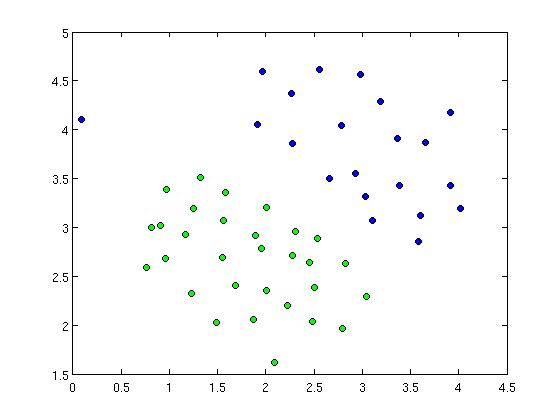
\includegraphics[width=.7\columnwidth]{twofeaturedata}
  \end{figure}
  %
  In this plot, we see two classes of data with a somewhat obvious separation gap. However, the blue class has an outlier on the far left. We'll now look at how this outlier affects the SVM decision boundary.




  \subsection{Setting Cost to $C = 1$}
  %
  Recall from the lecture videos that the parameter $C$ in the SVM optimization problem is a positive cost factor that penalizes misclassified training examples. A larger $C$ discourages misclassification more than a smaller $C$.

  First, we'll run the classifier with $C = 1$. To train your model, call
  %
  \begin{lstlisting}
    model = svmtrain(trainlabels, trainfeatures, '-s 0 -t 0 -c 1');
  \end{lstlisting}
  %
  The last string argument tells LIBSVM to train using the options
  %
  \begin{itemize}
    \item[a.] -s 0, SVM classification
    \item[b.] -t 0, a linear kernel, because we want a linear decision boundary
    \item[c.] -c 1, a cost factor of 1
  \end{itemize}
  %
  You can see all available options by typing ``svmtrain'' at the Matlab/Octave console.

  After training is done, ``model'' will be a struct that contains the model parameters. We're now interested in getting the variables $w$ and $b$. Unfortunately, these are not explicity represented in the model struct, but you can calculate them with the following commands:
  %
  \begin{lstlisting}[language=C, basicstyle=\footnotesize, showspaces=false]
    w = model.SVs' * model.sv_coef;
    b = -model.rho;
    if (model.Label(1) == -1)
        w = -w; b = -b;
    end
  \end{lstlisting}
  %
  Once you have $w$ and $b$, use them to plot the decision boundary. The outcome should look like the graph below.
  %
  \begin{figure}[htb!]
    \centering
      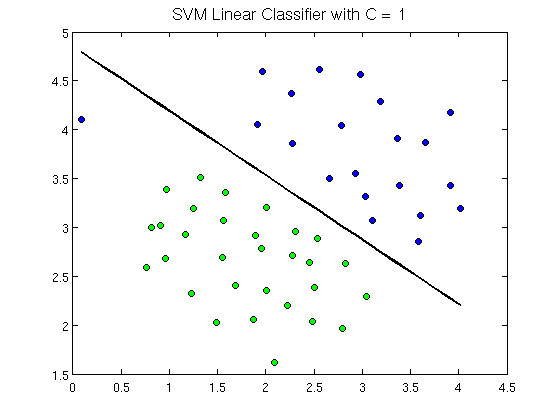
\includegraphics[width=.7\columnwidth]{twofeature_a}
  \end{figure}
  %
  With $C = 1$, we see that the outlier is misclassified, but the decision boundary seems like a reasonable fit.


  \subsection{Setting Cost to $C=100$}
  %
  Now let's look at what happens when the cost factor is much higher. Train your model and plot the decision boundary again, this time with $C$ set to 100. The outlier will now be classified correctly, but the decision boundary will not seem like a natural fit for the rest of the data:
  %
  \begin{figure}[htb!]
    \centering
      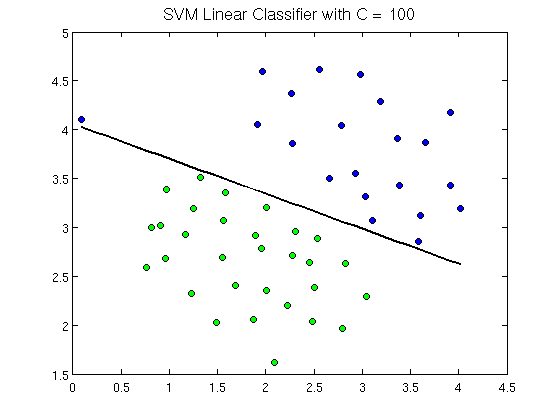
\includegraphics[width=.7\columnwidth]{twofeature_b}
  \end{figure}
  %
  This example shows that when cost penalty is large, the SVM algorithm will very hard to avoid misclassifications. The tradeoff is that the algorithm will give less weight to producing a large separation margin.



\section{Text classification}
%
  Now let's return to our spam classification example from the previous exercise. In your data folder, there should be the same 4 training sets you saw in the Naive Bayes exercise, only now formatted for LIBSVM. They are named:
  %
  \begin{itemize}
    \item[a.] email\_train-50.txt (based on 50 email documents)
    \item[b.] email\_train-100.txt (100 documents)
    \item[c.] email\_train-400.txt (400 documents)
    \item[d.] email\_train-all.txt (the complete 700 training documents)
  \end{itemize}

  You will train a linear SVM model on each of the four training sets with  $C$ left at the default SVM value. After training, test the performance of each model on set the named ``email\_test.txt''. This is done with the ``svmpredict'' command, which you can find out more about by typing ``svmpredict'' at the MATLAB/Octave console.

  During test time, the accuracy on the test set will be printed to the console. Record the classification accuracy for each training set and check your answers with the solutions. How do the errors compare to the Naive Bayes errors?






\end{document}
